
% ***************************************************
% Example of an internal chapter
% ***************************************************
%This is an internal chapter of the thesis.
%If you have a long title, you can supply an abbreviated version to print in the Table of Contents using the optional argument to the \chapter command.
\chapter[Design overview]{Design overview}
\label{chap:methodology}	%CREATE YOUR OWN LABEL.
\pagestyle{headings}

This chapter details the design decisions and steps taken to complete the project. The project itself can be broken down into three main areas: hardware, firmware and software. 


\section{FPGA}
Digilent, parented by National Instruments, make a wide range of Xilinx based FPGA development boards and test equipment. In this project, the Digilent Nexys A7-100T FPGA development board (figure \ref{fig:fpga_dev_board}) was used due to it's availability and features including: a Xilinx Artix 7 100T FPGA (part number XC7A100T-1CSG324C), LAN8720A 100MBit/s RMII PHY and PMOD (auxiliary outputs) amoung other IO. 

Xilinx has multiple FPGAs in their 7-series lineup with different target audiences. The Artix-7 family is optimised for low power designs with high logic throughput. The XC7A100T has 101,440 logic cells, 4,860Kbits of Block RAM (BRAM) and 240 DSP blocks \cite{Xilinx7SeriesDatasheet}. 


\begin{figure}[h!]
    \centering
    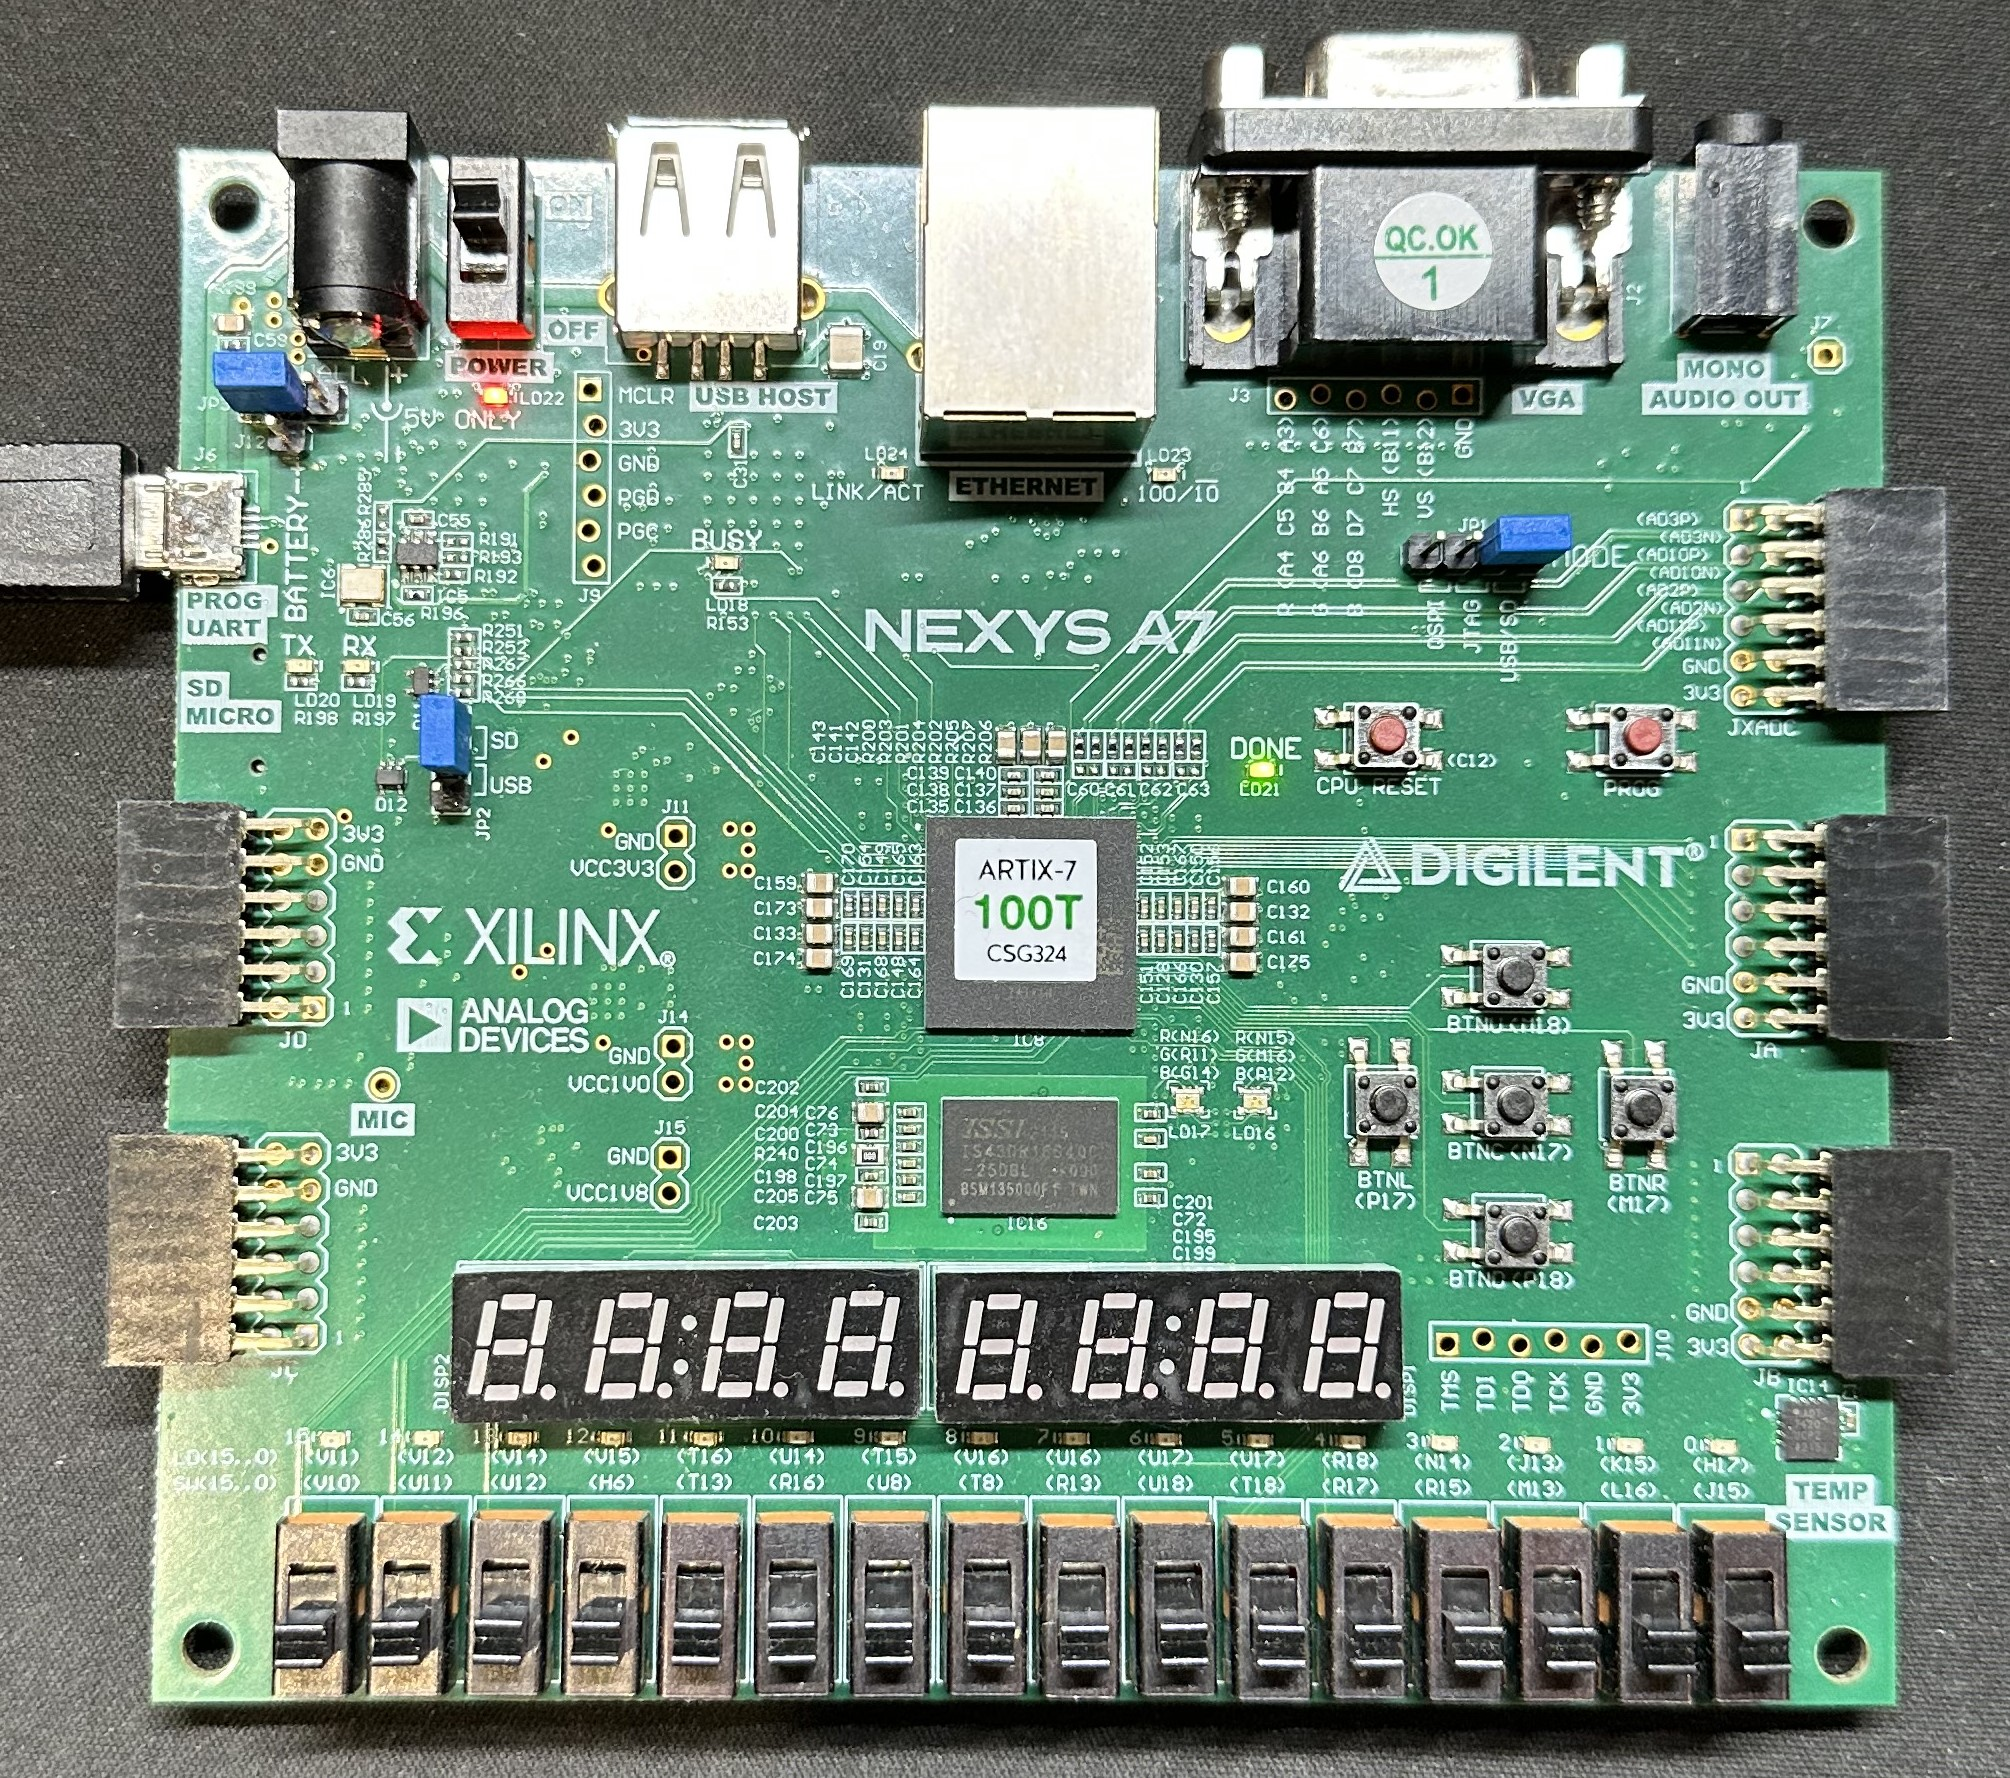
\includegraphics[width=0.65\textwidth]{Images/nexysa7_board.jpg}
    \caption[Digilent Nexys A7 FPGA development board]{Digilent Nexys A7 FPGA development board.}
    \label{fig:fpga_dev_board}
\end{figure}

\newpage




\subsubsection{PMOD Interface}

There are 5 PMOD connectors on the development board. Initally, one of these would be used for a second Ethernet PHY, but due to bandwidth limitations of the interface, the design had to be altered. The recommended bandwidth of these ports are 25MHz while the Ethernet RMII PHY would have been using 50Mhz signals over the interface. As such, signal integrity issues arose and could be seen in figure \ref{fig:eye_diagram} and restricted the use to just one interface - the onboard PHY. A new development board with two PHYs would be needed.

\begin{figure}[h]
    \centering
    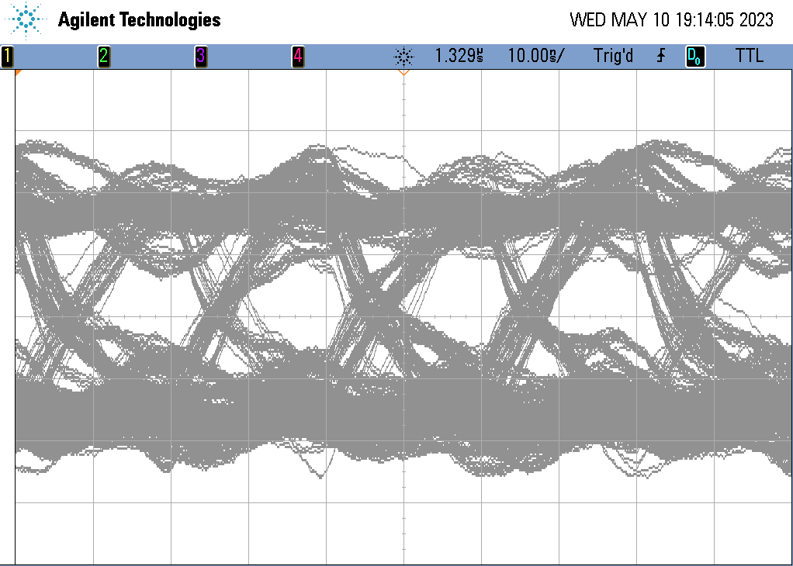
\includegraphics[width=0.65\textwidth]{Images/EyeDiagramTX.png}
    \caption[Eye diagram of TXD through PMOD interface]{Eye diagram of TXD through PMOD interface.}
    \label{fig:eye_diagram}
\end{figure}






\section{System on Chip}

The NEORV32 processor by GitHub user stnolting was used in this project. It's a highly configurable microcontroller-like SoC. 









\subsection{MicroSD card}
The web assets were stored on a MicroSD card. SD cards have 2 modes of operation: native SD mode and SPI mode. To keep things simple, the microSD card was connected to with SPI mode. 




\section{Ethernet Media Access Controller}
The advantage of using an FPGA is that custom hardware can be designed for specific tasks. In this design the MAC layer was done purely in hardware to free up the microprocessor by handling all of the lower level logic. 

This MAC was implemented as a memory-mapped perhipheral which used the MCU's Wishbone B4 classic interface. This then made it easily accessable over the memory address space of the MCU.  



\section{Packet Classifier}

To further save MCU resources, the packet classification was done in hardware. Not only did this reduce the load on the MCU itself - giving it more time to do other things - it allowed the interface to run at \textit{'wirespeed'}. That is, at the full speed of the interface - 100Mbit/s. 

This was possible by having the rulset been evaluated in parallel as the data is coming into the firewall. This method however is not suitable for large rulesets as the fan-in and fan-out limit the maximum number of parallel comparisons. For every new rule, the number of gates grows exponentially. Hence a design decision of a maximum ruleset of size 8 was chosen. 

The way this classifier was designed was to be a \textit{'default-block'} where all connections were blocked except for the ones specifically whitelisted in the ruleset. 

The specific rules had a few options, namely the source IP address, destination IP address, source port, destination port and protocol could be configured. In addition to these, each field had a wildcard operator which allowed all values for that specific option to be classified. 

A block diagram of the classifier can be seen in figure XX below. To control the flow of the packets, a buffer was used on the input to store the packet as it was coming in. At the same time the classifier would start classifying the packet. If allowed, then the packet would be moved on to another buffer before been sent out the other interface. If the packet was blocked, then the data would be dropped by clearing the buffers and then just ignoring the remainder of the incomming packet. 



To do the filtering itself, a shift register can be used to essentially delay the inputs from the RMII PHY until the packet classifier has determined whether to forward or drop the packet. A simple MUX can then be used to either allow the packet to enter the wishbone MAC or to not. 

As the hardware in the MAC only processes the input if crs\_dv is high, we only need to gate the crs\_dv and can always have the rxd lines always attached. Howerver, these should also go through a shift register.

By doing this, it means that we can operate the filter at wirespeed with the only downside is the extra latency that the shift registers bring. The delay that these registers add to the latency can be found to be $T_{latency} = N\times T_{clk}$ where $N$ is the size of the registers. In the design a size of 224 ticks was used. The thought process behind this was that at a minimum, the packet classifier needed to input a maximum of $22 + 24 + 4 = 50$ bytes (22 for MAC headers including preamble, maximum 24 bytes for IP header and 4 bytes for the TCP/UDP headers (only need to check the source and destination port)) need to be processed. While this is enough, a margin of 6 bytes was arbitarily chosen to allow propogation of other parts of the design to have taken effect. This gave 56 bytes, where each byte takes 4 clock cycles to input into the MAC meaning that we need a register size of $56 \times 4=224$ for the data to propagate to the end of the registers after the packet classifier has determined whether to drop or allow the packet. This means that at a clock frequency of 50Mhz, the added latency is $224 \times \frac{1}{50\times 10^6} = 4.48 \times 10^{-6} = 4.48uS$.

Importantly this does not effect the speed/bandwidth of the connection. 



\section{Firmware}


\subsection{Drivers}
\subsubsection{Ethernet drivers}
Since the ethernet hardware was custom, drivers were needed to interface with the hardware in software. There were two types of commands that were needed, first the RMII serial managment interface (SMI) and secondly the MAC drivers - the drivers that would handle the data.  The SMI interface is used to control the mode of operation of the PHY chip including the speed, Auto-MDIX, duplex settings. The LAN8720A datasheet, (\cite{LAN8720ADatasheet}) provided some details (seen in figure \ref{fig:smi_packet_structure}) into how the protocol operated. The datasheet also outlined that a maximum frequency of 2.5MHz, but no lower bound. As such the interface was \textit{'bitbanged'} to reduce complexity. The maximum switching frequency of the NEORV32's GPIO was measured to be $\approx 1$MHz, thus the interface could operate without any additional delays.


\begin{figure}[h!]
    \centering
    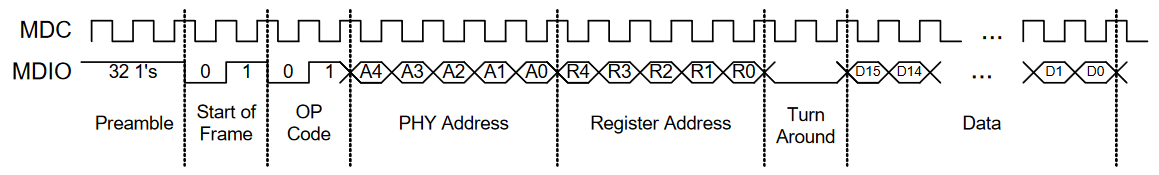
\includegraphics[width=0.75\textwidth]{Images/SMIWriteStructure.png}
    \caption[SMI Write message structure]{SMI Write message structure. \cite{LAN8720ADatasheet}}
    \label{fig:smi_packet_structure}
\end{figure}


As the Ethernet hardware used the Wishbone interface, the register locations were mapped into the processors address space. Simple macros can be created for ease of use. 

\begin{lstlisting}[language=C, caption=Python example]
#define ETH_MAC_TX_BASE 0x13371000
#define ETH_MAC_CMD_BASE 0x13370000

#define ETH_MAC_CMD  (*(volatile uint32_t *)ETH_MAC_CMD_BASE)
#define ETH_MAC_TX ((EthMacTx *) ETH_MAC_TX_BASE)

typedef struct __attribute__((__packed__))  {
    volatile uint32_t SIZE;
    volatile uint32_t DATA[375]; // 1500 / 4 = 375.
} EthMacTx;
\end{lstlisting}

\subsubsection{SD card drivers}
As part of the documentation for the FreeRTOS-Plus-FAT file system, drivers for the media was required. Like the Ethernet hardware, the driver had to implement at least three functions: function that reads sectors from the media, one that rights sectors to the media and one to initialise the media. 




\section{Software}



\subsection{Real Time Operating System}
In addition to simplifying the project, and RTOS was used as this would allow the use of network TCP stacks. The RTOS that was used in this design was FreeRTOS V10.4.4 due to its familirity and compatability with the NEORV32 MCU.


\subsection{Network Stack}
There were two main options for the network stack, LwIP and FreeRTOS-Plus-TCP. The main concern with LwIP was that it was not threadsafe and had memory issues. In addition to this, as FreeRTOS was chosen as the RTOS, their own TCP stack was used as it was thought to have tighter integration. 


\subsection{Webserver}
A simple HTTP webserver running on top of a TCP server was used to serve the webpages for the project. 

HTTP runs on top of TCP, as such, a TCP server was first created which handled all the TCP handshaking and then allowed HTTP data to be sent over the socket. The HTTP server would then process this data, access the filesystem if needed and respond on the socket. 


\subsubsection{API server}
A subset of the webserver is the API server itself. To make the design simpler, an API was created so that the interface to set and get the firewall rules was independant of the web content.

For setting the firewall rules, a POST request to the \textit{'/api/firewall'} endpoint could be made. The body of the request would contain the rule in the following format

\[
payload=Index | Wildcard | IP_{Dest} |  IP_{Src}  | Port_{Dest} |  Port_{Src} | Protocol
\]

Where $|$ is the concatination operator and all fields are in hexadecimal. As an example, to insert a rule at index 0, and with a wildcard operator for all items with a destination IP of 10.20.1.120, source IP of 10.0.0.159, source and destination port of 80 and a protocol of TCP, the following body would need to be sent to the API: \textit{'payload=003F0A1401780A00009F0050005006'}.

This would then be decoded in the webserver itself and applied to the packet filter. 




\subsection{Command line interface}


\subsection{Improvements}

\begin{itemize}
    \item Bidirectional filtering - currently only doing incomming filtering
\end{itemize}